\documentclass{BYUTextbook}

% The \lipsum command just loads dummy text.
\usepackage{lipsum}

\begin{document}

\frontmatter

\thispagestyle{empty}
\begin{adjustwidth}{}{-1.5in}

 \centering
 \vspace{1in}
 \Huge The BYUTextbook Class
 \normalsize
 \vspace{1in}

 Justin Peatross

 Michael Ware

 Brigham Young University

 \vspace{1in}

\today

\vspace{1in}

Sometimes you will want to center things on the page rather than
between the margins, since the margin is big to make room for
figures.  This page shows how to do that.

\end{adjustwidth}

\cleardoublepage

\tableofcontents

\mainmatter

\chapter{An Example Chapter}

General Notes:
\begin{itemize}
  \item Many of the commands and  environments need several
      runs of \LaTeX to get the formatting right.  If something
      looks weird, try compiling several more times.
  \item The margin figure and inline figure commands set the
      label of the figure to be the same as the file name.
\end{itemize}
We are still cleaning up and improving as we go along.  The
following shows examples of several of the environments that can be
created.  Feel free to modify the code and use as you like, but
change the name if you do.

\section{Equation Notes}
\label{sec:EqNotes}

Notes can be put inside the equation by the number
\begin{equation}
    E=mc^2, \numnote{(Einstein's famous equation)}
\end{equation}
inside the equation by the equation
\begin{equation}
    E=mc^2, \innote{\qquad (Einstein's famous equation)}
\end{equation}
or out in the margin
\begin{equation}
    E=mc^2, \outnote{(Einstein's famous equation)}
\end{equation}


\section{The Example Environment}

The example environment is designed for displaying a sample problem
and then a sample solution.  It is set off from the main text with
a vertical bar that runs next to the problem

\begin{example}
    \exProblem
    How much wood could a woodchuck chuck if a woodchuck
    could chuck wood? \label{example:One}
    \exSolution
        \lipsum[6]
\end{example}

In Example~\ref{example:One}, we illustrated how to make the
example environment. Page breaks can be awkward and sometimes need
some manual intervention.

\section{The Derivation Environment}

The derivation environment sets of a chunk of text with a vertical
bar and gives it a title.  We use it to set of derivations that get
in the way of readability.
\begin{derivation}{This derivation is offset from the text}
        \lipsum[6-7]
\end{derivation}

\section{Margin Figures}

\marginfig[-2in]{f01Faraday}{Faraday's law.\label{fig:George}}

We've found that it is easier to keep figures near the appropriate
place in the text if they are put in the margin next to the
paragraph.  The marginfig command does this, as in
Fig.~\ref{f01Faraday}.  By default, the figure is placed right next
to the text where the command is located, but sometimes you need to
move it.  There is an optional length argument for that moves the
figure up or down.  The first required argument is the file name,
and by default the filename is also used as the label.  You can
also give your own label in the caption text, as shown in the code
for Fig.~\ref{fig:George} if you don't like this convention.

\section{Inline Figures}
If you want inline figures right where you put the command, use
inlinefig.

\inlinefig{f03ReflectanceLab}{Experimental setup.}

This command can have awkward page breaks if you aren't careful,
but can be useful especially in problems.  As before, the default
label is the file name, but you can choose your own if you don't
like it.

\section{Wide Figures}

\begin{figure}[b]
    \inneralign{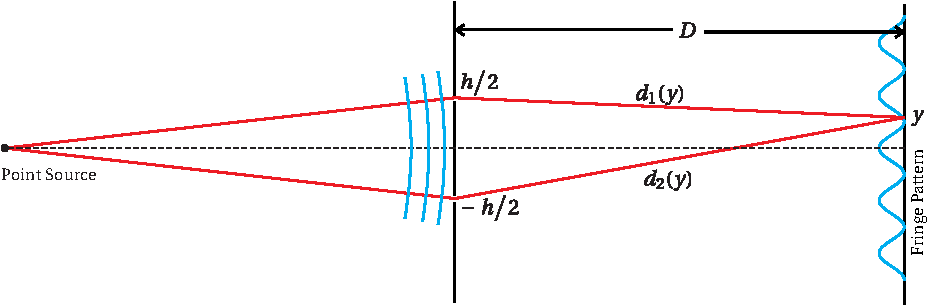
\includegraphics{f08Young}}
    \caption{\label{fig:8.6} A point source produces coherent
    (locked phases) light.  When this light which traverses two
   slits and arrives at a screen it produces a fringe pattern.
    }
\end{figure}


Regular figures can be included as usual.  If you need an extra
wide figure that extends in the margin, you can use the
hacked-together inneralign command to get it to extend into the
correct margin.  (Several compilations may be necessary to get it
to realize which margin is correct.  This construction is
illustrated in Fig.~\ref{fig:8.6}.



\section{Person Feature}

We think science is more interesting if you can put it in a
personal context.  Sometimes you can do this in the text, but
sometimes it is nice to have a picture and some basic facts.  The
personfeature command will do this for you.  Since these may need
to be vertically adjusted to avoid margin figures or page breaks,
there is an optional length argument.

\personfeature[-1in]{f00Descartes}{Ren\'{e}
    Descartes}{1596-1650, French}{was born in  in La Haye en
    Touraine (now Descartes), France. His mother died when he was
    an infant.  His father was a member of parliament who
    encouraged Descartes to become a lawyer. Descartes graduated
    with a degree in law from the University of Poitiers in 1616.
    In 1619, he had a series of dreams that led him to believe that
    he should instead pursue science.  Descartes became one of the
    greatest mathematicians, physicists, and philosophers of all
    time.  He is credited with inventing the cartesian coordinate
    system, which is named after him.  For the first time,
    geometric shapes could be expressed as algebraic equations.
    \href{http://en.wikipedia.org/wiki/Rene_Descartes}{(Wikipedia)}}



\section{Code Listings}

We typeset code for several lab manuals using this class.  We have
the class set up so that it writes a sample code file with a Matlab
extension (.m) as well as displaying it.  Then we can post the
sample code files with the manual.  This is illustrated in
Listing~\ref{listing:1}.  For now, everything is hardcoded for
Matlab syntax formatting and file names.\index{Code Listings}
\begin{codeexample}\label{listing:1}
\begin{VerbatimOut}{\listingFile}
clear; close all;

N=100;

a = zeros(1,N);
% Fill the a array
for n=1:N
    a(n) = 1 / n^2;
end

S = zeros(1,N);
% Do the running sum
for m=1:N
    S(m) = sum( a(1:m) );
end

% Now let's plot S vs. m
m=1:N
plot(m,S)
\end{VerbatimOut}
\end{codeexample}

You can override the auto-naming convention as in
Listing~\ref{listing:2}
\begin{codeexample}[DisplayPi.m]\label{listing:2}
\begin{VerbatimOut}{\listingFile}
clear;
close all;

% This is how you display the value of pi
pi
\end{VerbatimOut}
\end{codeexample}

% Make the problems section

\section{Margin Notes}

You can make little margin reminder notes with a character bullet
of your choice using the reminder command, like this:

\reminder{\lefthand}{A reminder is basically just a marginpar with
a little icon next to it.}

For a list of icons, see the Fourier package documentation.  (That
package defines the font and character set for this
class).\index{Fourier}

\section{Margin Tables}

Sometimes it is nice to put data in the margins in tabular form.
Table~\ref{tab:Radiometric} is an example of a text table, and you
can put numbers and equations in such a table too.  Obviously the
data has to fit well in the narrow form factor.  As with the other
margin elements, there is an optional length argument to adjust
vertical position.  The required height argument specifies the size
of the colored box.

\columntable[-0.75in]{4.1in}{
    \textbf{Radiant Power (of a source):}  Electromagnetic energy.
    Units: $\mathrm{W}=\mathrm{J}/\mathrm{s}$

    \medskip

    \textbf{Radiant Solid-Angle Intensity (of a source):} Radiant power
    per steradian emitted from a point-like source ($4\pi$ steradians
    in a sphere). Units:  $\textrm{W} / \textrm{Sr}$

    \medskip

    \textbf{Radiance or Brightness (of a source):} Radiant solid-angle
    intensity per unit projected area of an extended source. The
    \emph{projected} area foreshortens by $\cos \theta$, where $\theta$
    is the observation angle relative to the surface normal. Units:
    $\mathrm{W} / (\mathrm{Sr}\cdot \mathrm{cm}^2)$

    \medskip

    \textbf{Radiant Emittance or Exitance (from a source):} Radiant
    Power emitted per unit surface area of an extended source (the
    Poynting flux leaving). Units: $\mathrm{W} / \mathrm{cm}^2$

    \medskip

    \textbf{Irradiance (to a receiver) Often called intensity:}
    Electromagnetic power delivered per area to a receiver: Poynting
    flux arriving. Units: $\mathrm{W} / \mathrm{cm}^2$
    }{Radiometric quantities and
    units.\label{tab:Radiometric}}

\ExSection[Exercises]

The exercise section is designed to organize problems by section,
like this

\begin{exercises}{sec:EqNotes}

\prob{FileName} A hard problem \label{prob:hard}

\lab Measure the thing in P~\ref{prob:hard}.
\end{exercises}

 \cleardoublepage \phantomsection
 \addcontentsline{toc}{chapter}{Index}
 \RaggedRight
 \thispagestyle{empty}
 \printindex


\end{document}
